% PART III — PROJECT ARCHITECTURE AND DEVELOPMENT
\chapter{Chapter 4: Modular System Stack, Simulation Design, and Engineering Verification}
\section{4.1 Four-Layer Robotics Architecture and Authoritative PyBullet Core}
Across 17 research phases and subsequent full-stack refactoring, the platform converged onto four decoupled architectural planes (Figure 4.1): (1) Physics Simulation Core (PyBullet 240 Hz engine paired with MuJoCo 4.0.1 MJCF parity validator); (2) Robotics Kinematics, Perception \& Controllers (`robotics/robots/franka\_panda/`, `src/controllers/`, `src/perception/`, `src/rl/adaptive\_controllers.py`); (3) Goal-Conditioned Gymnasium/HER Task Suites (`PandaReachEnv` through `PandaContactAssemblyEnv`); and (4) Training/Workstation Execution (`SB3`, `BCDecayingSAC`, `FastAPI SimulationManager`, `React + Three.js` digital twin).

\begin{figure}[htbp]\centering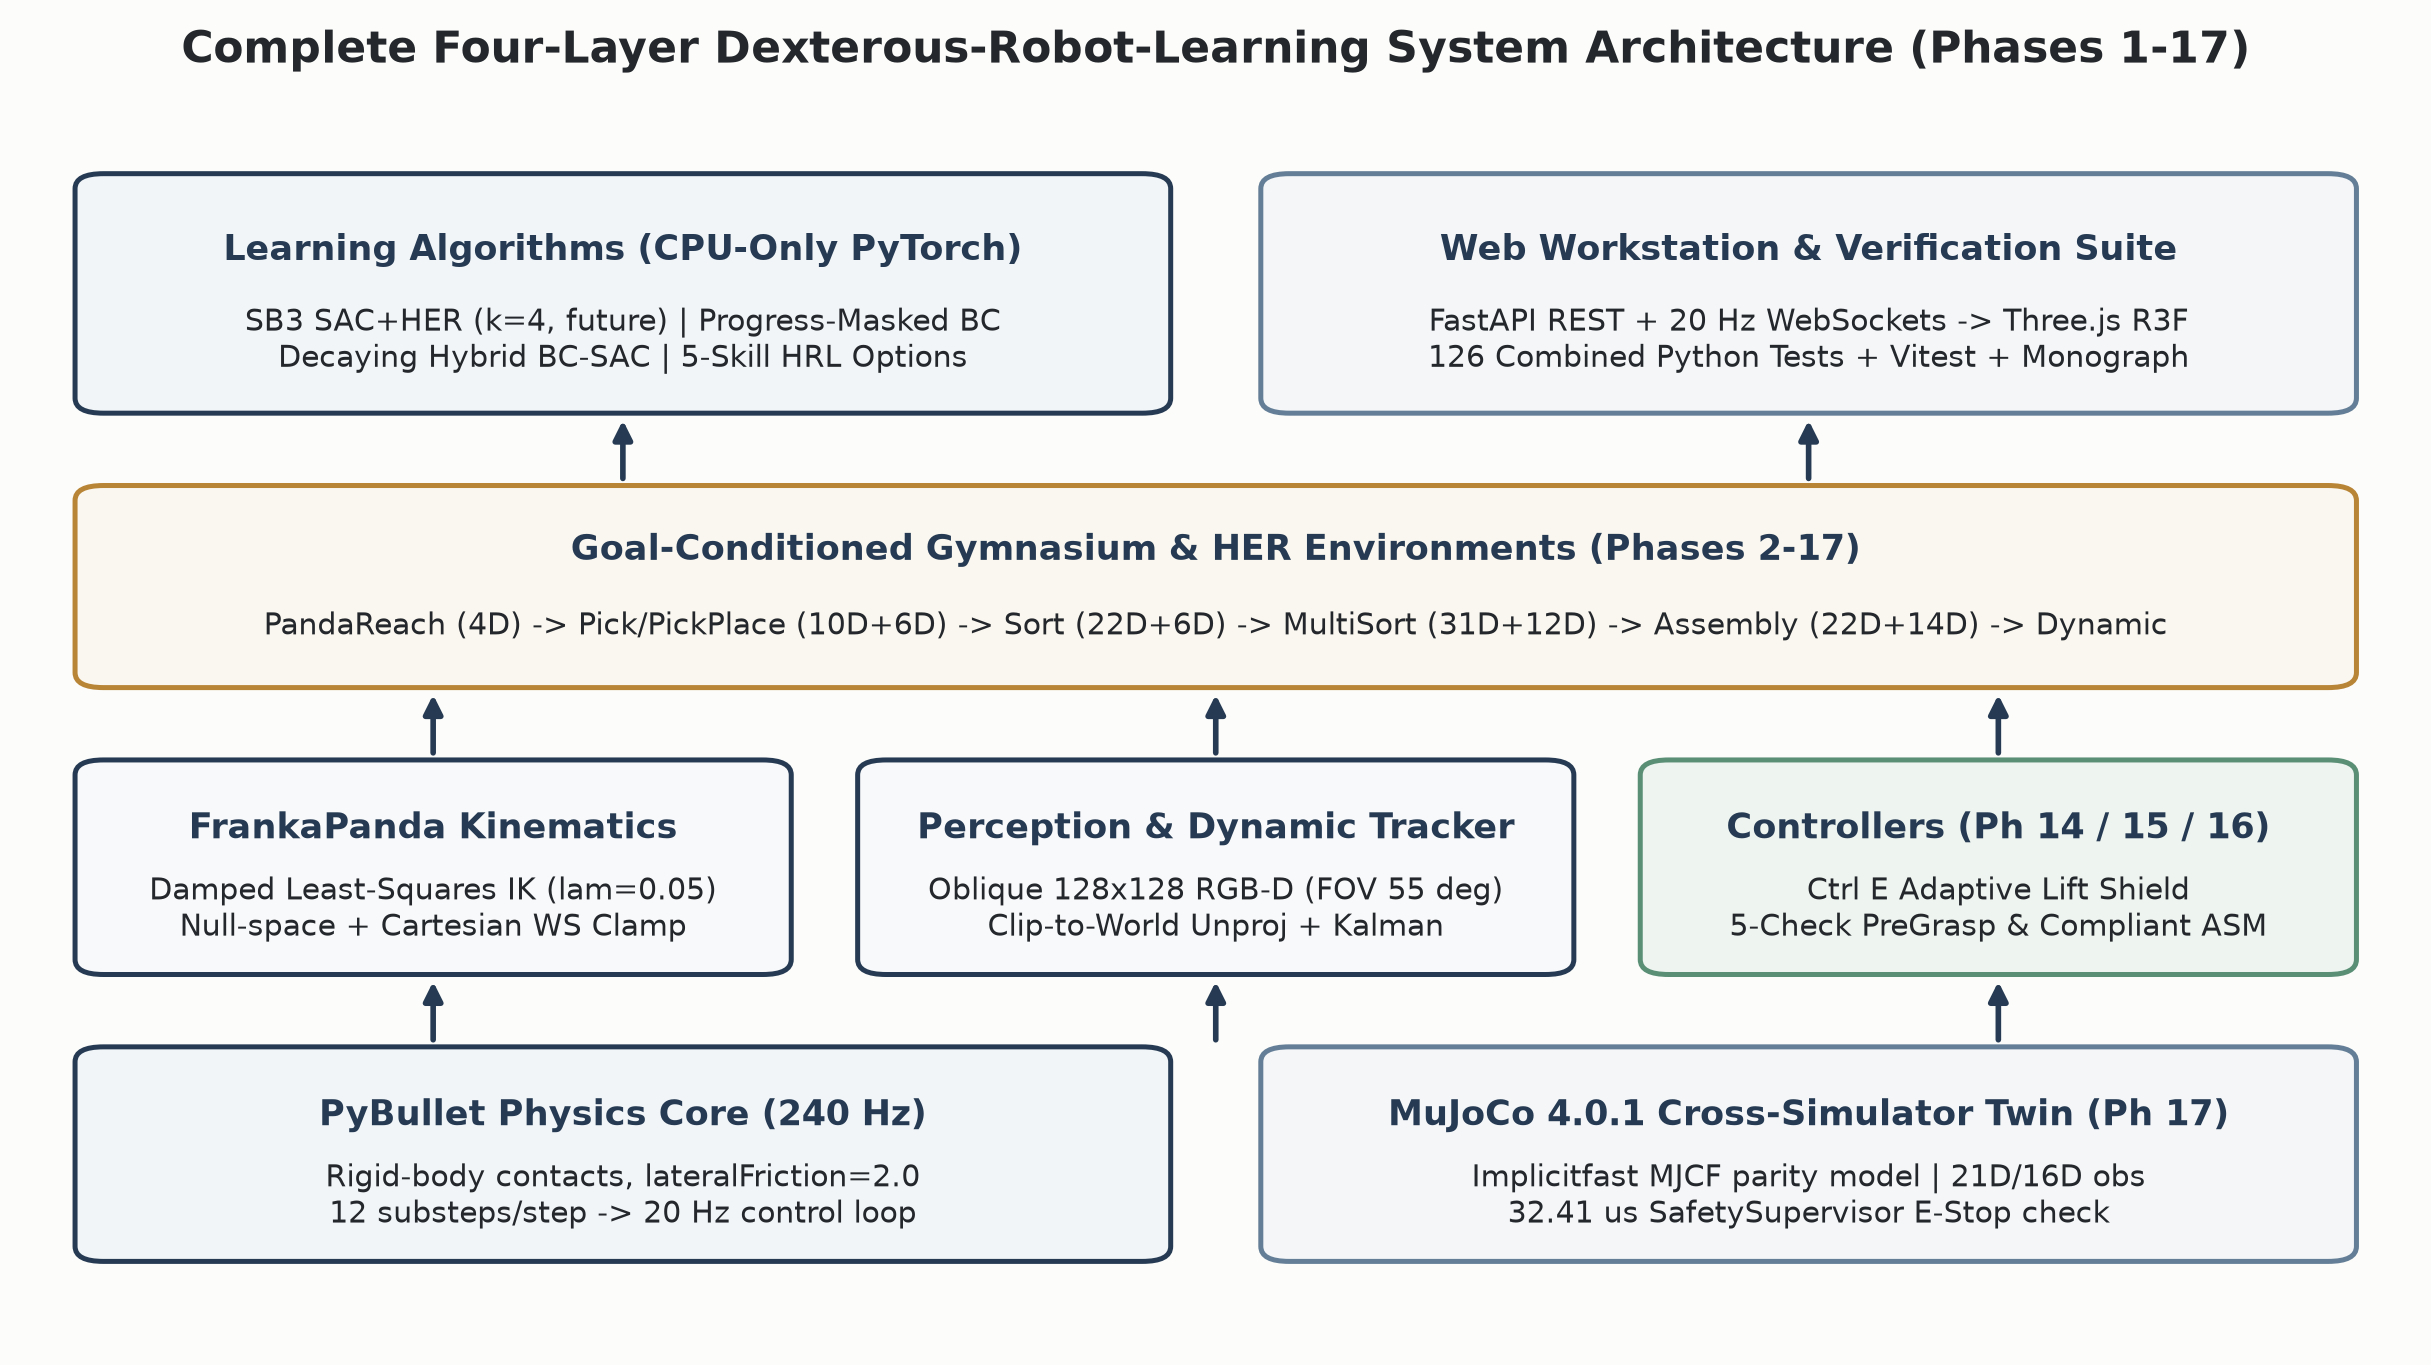
\includegraphics[width=0.9\linewidth]{../../assets/diagrams/diag_01_system_architecture.png}\caption{Figure 4.1: Complete four-layer Dexterous-Robot-Learning architecture unifying physics, control, RL/perception, and web workstation.}\end{figure}
\begin{figure}[htbp]\centering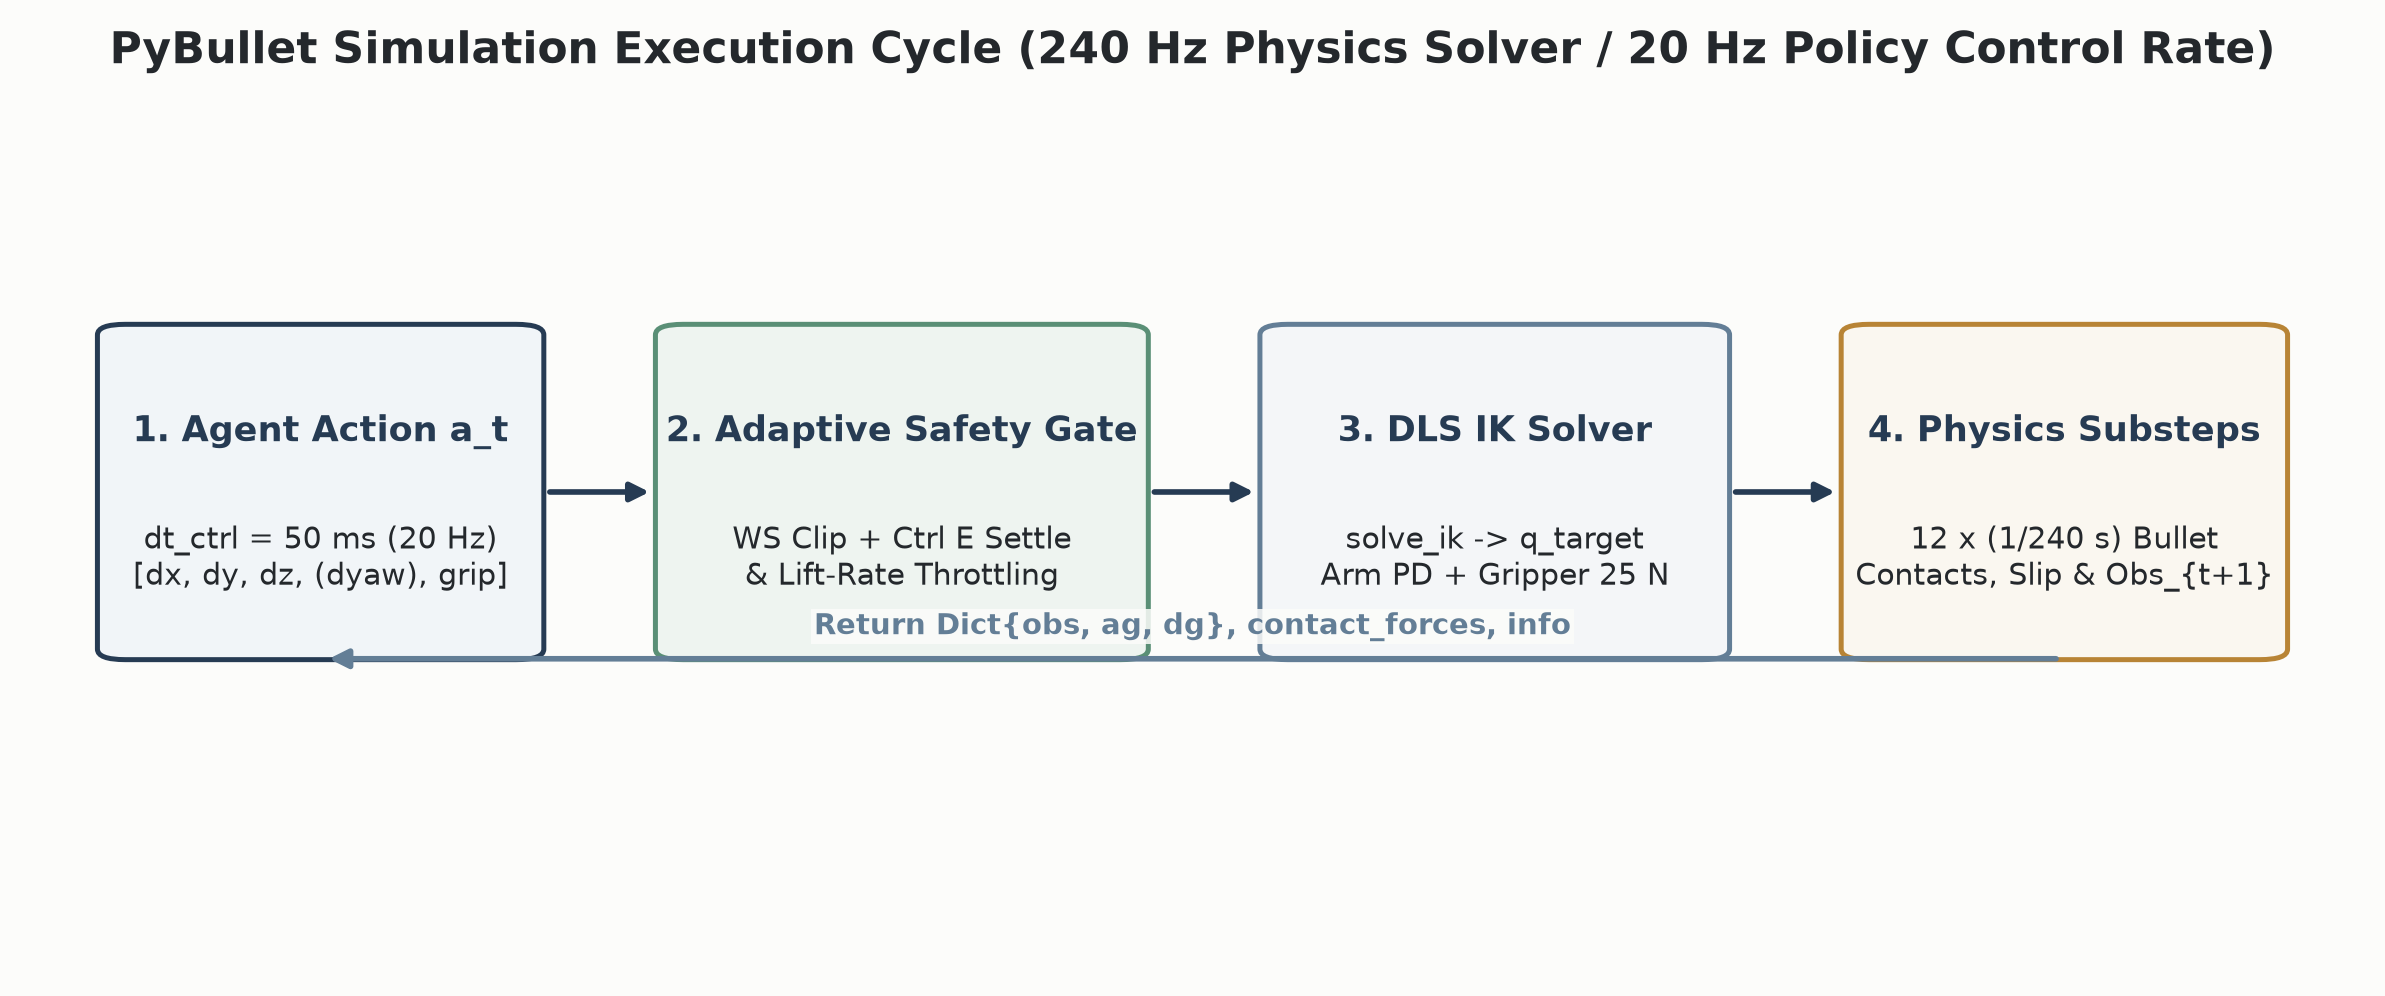
\includegraphics[width=0.9\linewidth]{../../assets/diagrams/diag_02_pybullet_sim_loop.png}\caption{Figure 4.2: Authoritative PyBullet 240 Hz stepping cycle, adaptive lift guard, DLS IK projection, and 20 Hz observation broadcast.}\end{figure}
\section{4.2 Environment Dimensionality \& Verification Discipline}
A key engineering strength is zero silent assumption about tensor dimensions. Live environment introspection verifies exact observation, goal, and action spaces: `PandaReachEnv` exposes `(4,)` observation + `(3,)` achieved/desired goals (`10D` total Dict); `PandaPickEnv`, `PandaPickPlaceEnv`, `PandaDynamicPickPlaceEnv`, and `MuJoCoPandaPickPlaceEnv` share `(10,)` + `(3,)+(3,)` (`16D` Dict); `PandaSortEnv` and `PandaSinglePreGraspEnv` expose `(22,)` + `6D` (`28D` Dict); `PandaMultiSortEnv` / `PreGrasp` expose `(31,)` + `(6,)+(6,)` (`43D` Dict); and assembly environments expose `(22,)` + `(7,)+(7,)` `SE(3)` pose goals with 5D `[dx, dy, dz, dyaw, gripper]` actions. The automated regression suite expanded monotonically from 37 tests (Phase 1) -> 52 (Phase 9) -> 56 (Phase 10) -> 111 (Phase 15) -> 126 combined Python + backend integration tests today with zero skipped or relaxed assertions.

\begin{longtable}{l l l l l l}\caption{Table 4.1: Verified Gymnasium \& Cross-Simulator Environment Contracts}\\\toprule
Environment Class & Obs & Goals (AG+DG) & Action & Horizon & Provenance / Phase \\ \midrule \endhead
PandaReachEnv & 4D & 3D + 3D & 4D & 50 & Phase 2 / Sparse Goal \\
PandaPickPlaceEnv / Dense & 10D & 3D + 3D & 4D & 100 & Phase 6 / 12–14 Core \\
PandaSinglePreGraspEnv & 22D & 3D + 3D & 4D & 80 & Phase 15.2.5B PreGrasp \\
PandaMultiSortPreGraspEnv & 31D & 6D + 6D & 4D & 300 & Phase 15.2.5A 2-Obj \\
PandaContactAssemblyEnv & 22D & 7D + 7D & 5D & 120 & Phase 15.3 / 16.4 ASM \\
PandaDynamicPickPlaceEnv & 10D & 3D + 3D & 4D & 100 & Phase 16.3 Kalman \\
MuJoCoPandaPickPlaceEnv & 10D & 3D + 3D & 4D & 100 & Phase 17.1 Cross-Sim \\
\bottomrule \end{longtable}